\documentclass[12pt]{article}
\usepackage[margin=2.5cm]{geometry}
\usepackage{graphicx}
\usepackage{amsmath}
\usepackage{amssymb}
\usepackage{booktabs}
\usepackage{float}
\usepackage{setspace}\onehalfspacing
\usepackage{caption}
\usepackage{titlesec}
\usepackage{hyperref}
\usepackage[ddmmyyyy]{datetime} % for changing the date format
\usepackage{multicol}
\usepackage[style=apa]{biblatex}
\usepackage{enumitem}
\usepackage{multirow}

\addbibresource{citation.bib}

% Redefine caption style
\DeclareCaptionFormat{underlined}{\underline{#1}#2#3}
\captionsetup[table]{format=underlined,labelfont=bf}
\captionsetup[figure]
{format=underlined,labelfont=bf}

\hypersetup{
    pdftitle={Thesis Report},
    pdfauthor={Adam Maghout},
    pdfsubject={Educational measurement},
    pdfkeywords={Education, International Baccalaureate, Measurement, IB, Resits, Retakes},
    bookmarksnumbered=true,     
    bookmarksopen=true,         
    bookmarksopenlevel=1,       
    colorlinks=true,            
    pdfstartview=Fit,           
    pdfpagemode=UseOutlines,      
    pdfpagelayout=TwoPageRight
}

% Set font size to 12pt
\renewcommand{\normalsize}{\fontsize{12}{13}\selectfont}

% Reduce spacing before and after section titles
\titlespacing*{\section}{0.5pt}{*0.2}{*0.4}
\titlespacing*{\subsection}{0.5pt}{*0.6}{*0.6}
\titlespacing*{\subsubsection}{0.5pt}{*0.4}{*0.6}

% Reduce spacing in the list environment
\setlength{\itemsep}{0.6pt}
\setlength{\parskip}{1.2pt}
\setlength{\parsep}{1pt}

\begin{document}

\title{Evaluating the Impact of Passing Criteria and Retakes on Misclassification in the IB Diploma Programme}
\begin{spacing}{1.5}
\begin{titlepage}
    \centering
    {\LARGE \textbf{Evaluating the Impact of Passing Conditions and Retakes on Misclassification in the IB's Diploma Programme}\par}
    \vspace{1.5cm}
    {\Large Adam Maghout\\Student number: 7692617\par}
    \vspace{1.5cm}
    {\large \textit{Course: Methodology and Statistics for the \\Behavioural, Biomedical and Social Sciences
    \\~\\Supervisor: Anton Béguin\\(International Baccalaureate)}\par}
    \vspace{0.5cm}
    \begin{multicols}{2}
    {\large Word count: 2485\\FETC approval: 24-2025\par}
    \columnbreak
    {\large Due date: 22/12/2024\\Submission date: \today\par}
    \end{multicols}

    \vspace{0.5cm}
    
\includegraphics[scale=0.2]{Photos/IB Logo.jpg}
    \vspace*{\fill}
\end{titlepage}
\end{spacing}
\newpage

\section{Introduction}

International assessment studies such as PISA have had a lasting impact on how education systems are perceived (\cite{waldowWhatPISADid2009}). Beyond improving cross-country performance, the quality of tests carries significant financial, legal and psychological implications, with suicide attempts spiking in recent years during exam periods (\cite{georgeExamSeasonStress2024}). 

Thus, when the cost of assessments for students is substantial, for example with school leaving exams, it is good practice not to rely on a single exam score for pass/fail decisions, as suggested in the Standards for Educational and Psychological Testing (\cite{americaneducationalresearchassociationStandardsEducationalPsychological2014}). Instead, a composite approach is favoured, wherein a decision rule defines the combination of multiple test results used to make the pass/fail decision.

The International Baccalaureate Organisation (IB0) is a transnational non-profit that offers courses to globally mobile students aged 3 to 19 (\cite{dohertyAppealInternationalBaccalaureate2009}) and provides internationally recognised qualifications (\cite{kingInternationalStudentMigration2013}). Among these is the Diploma Programme (DP), offered since 1970 and akin to British A levels (\cite{dohertyAppealInternationalBaccalaureate2009}). As few analytical studies have assessed the quality of its measurement tools (\cite{hillInternationalBaccalaureateIB2014}), this study examined the precision of DP passing rules as part of an internal quality review designed to revise the passing criteria ahead of the 2032 exam session. 

Few quantitative evaluations of high-stakes passing criteria exist. This study drew on the work of van Rijn et al. (\cite*{rijnEducationalMeasurementIssues2014}), which examined the passing criteria precision within Dutch secondary education and found that compensatory rules reduced misclassification. Similarly, Yocarini et al. (\cite*{yocariniSystematicComparisonDecision2018}) conducted a comparison of passing decisions on a psychology bachelor’s program at Erasmus University Rotterdam.

While these studies considered measurement error at subject level, the impact of viewing measurement error at item level remains unexplored. Comparing both approaches here will thus inform future evaluations of other exam systems. Moreover, retakes in high-stakes contexts remain unexamined quantitatively. The purpose of retakes is twofold: giving non-proficient examinees the opportunity to improve their competency and correcting the grades of proficient examinees who previously failed (\cite{coggeshallExaminationClassificationAccuracy2021}). Therefore, this study also examined how retake exams in the DP influenced missclassification rates.

In sum, this research aimed to determine the extent to which current IB passing conditions accurately classify students and whether increased compensation is warranted through less stringent passing rules or additional opportunities for resits. Precision differences across countries and institution types were also analysed to inform targeted interventions.

\section{Background}

\subsection{Decision rules}

Composite decision rules require meeting multiple criteria for a favourable outcome. For example, requiring minimum grades in both mathematics and chemistry constitutes a composite decision rule, as the decision is reliant on two separate outcomes. Composite rules always outperform simple ones when tests are correlated (\cite{vermeulen-kerstensNominaalStuderenHet2012}) as similar constructs are being measured. This assumption is however often violated when excess ability in one subject cannot compensate deficiency in another (\cite{mehrensUsingCollegeGPA1989}).

Decision rules are typically conjunctive or compensative. Conjunctive rules require sufficient scores on all tests. Conversely, compensative rules only require a sufficient score on average (\cite{rijnEducationalMeasurementIssues2014}). This is illustrated in Figure \ref{fig:Decisions1}. 
% Commented out for conciceness but can be re-integrated later
% Lord (\cite*{lordCuttingScoresErrors1962}) notes that a conjunctive decision rule will always perform suboptimally when faced with observed scores because of measurement error, even if a conjunctive rule is assumed for the true scores. 
In practice, large-scale assessment rules often combine conjunctive and compensative aspects, which are referred to as complex decision rules (\cite{douglasEstimatingClassificationAccuracy2010}).

\begin{figure}[htbp]
    \centering
    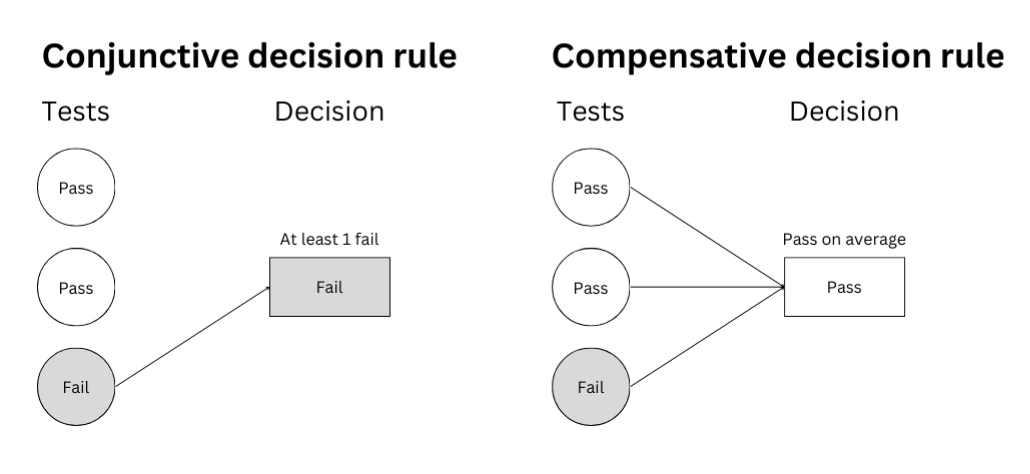
\includegraphics[scale=0.4]{Photos/Decision.jpg}
    \caption{Conjunctive and compensative decision rules.}
    \label{fig:Decisions1}
\end{figure}

\subsection{The Diploma Programme}

DP students are required to select six subjects, three or four taken at Higher Level (HL) and the remainder at Standard Level (SL) (\cite{tayMovementInternationalEducation2023}).
% Table \ref{tab:SubjectGroups} outlines the subject groups.
The exact options vary depending on the delivering institution and the country (\cite{maireIBDiplomaGlobalisation2021}). HL subjects explore material in greater depth, reflected in more contact hours and complex assessments. Subjects are graded from 1 to 7, with a 42-point maximum.

Completion of the DP core is also required, which includes three components: a project in Creativity, Activity, and Service (CAS), an Extended Essay (EE), and a Theory of Knowledge (TOK) component (\cite{tayMovementInternationalEducation2023}). Whilst CAS is assessed on a pass/fail basis, the EE and TOK are graded on a scale from A to E. Together, they award three additional points, bringing the maximum possible score for the DP to 45. Subject grades, including those for the core, are determined based on performance across multiple components. For instance, in biology, grades are derived from results on three examination papers and a practical assessment. An unattempted component yields an N. Students may also retake courses to pass or to improve a previous grade. Currently, six requirements govern the DP (\cite{DPPassingCriteria2023}):

% Commented out for conciceness but can be re-integrated later
% \begin{table}[ht!]
% \centering
% \renewcommand{\arraystretch}{1.3} % Add global vertical padding
% \caption{Subject Groups in the DP.}
% \label{tab:SubjectGroups}
% \begin{tabular}{ll}
% \hline
% \textbf{1} & Studies in Language and Literature \\
% \textbf{2} & Language Acquisition \\ 
% \textbf{3} & Individuals and Societies \\
% \textbf{4} & Sciences \\
% \textbf{5} & Mathematics \\
% \textbf{6} & The Arts \\
% \hline
% \end{tabular}
% \end{table}

\begin{itemize}[itemsep=0pt, parsep=0pt]
    \item[-] No fewer than 24 points in total, of which at least 12 at HL and 9 at SL. If only two SL subjects are taken, this last requirement is lowered to 5.
    \item[-] No N or E awarded on any subject, including TOK and EE.
    \item[-] No grade 1 awarded.
    \item[-] No more than two grade 2s awarded.
    \item[-] No more than three grade 3s or below awarded.
    \item[-] CAS requirements are met.
\end{itemize}

Most requirements are compensatory; for example, the 24-point minimum lets students offset a poor grade with a strong one. However, some aspects are deliberately conjunctive, preventing prioritisation of certain subjects over others. Though simplified in 2014, further simplification of the passing criteria is under consideration to maintain difficulty but reduce overlap between requirements. The present study seeks to evaluate the impact of modifying these rules on misclassification rates.

\subsection{Measurement precision}

In accordance with van Rijn et al. (\cite*{rijnEducationalMeasurementIssues2014}), the notion of measurement precision used here stems from the Classical Test Theory (CTT) framework. For a single test, a participant's observed score $X$ is given by a true score $T$, and an error term $E$ related to person and test characteristics:

\begin{equation}
\label{eqn:obstrue}
    X=T+E
\end{equation}

The goal is to ensure $X$ closely approximates $T$, effectively minimising $E$. The extent to which this is achieved is quantified by the test's reliability, which is the main measure of precision in CTT. Common reliability indicators include Cronbach's $\alpha$ (\cite{cronbachCoefficientAlphaInternal1951}) and McDonald's $\omega_t$ (\cite{mcdonaldTestTheoryUnified1999}), both measures of internal consistency. They are related to the systematic measurement error of a test:

\begin{equation}
\label{eqn:rel}
    SE_{meas}=\sigma_X\sqrt{1-R}
\end{equation}

\noindent
where $\sigma_X$ is the standard deviation of the test scores. Thus, if a decision rule is applied on the basis of a single test, the misclassification rate will depend on the reliability. Misclassification is defined here as students being assigned the wrong passing decision given their test scores, where the true passing decision is obtained by applying the decision rule to the unobserved true scores. The issue then becomes estimating the true scores, which can be done using simulation-based methods. 

Although methods for creating composite scores exist (\cite{gulliksenTheoryMentalTests1950}), these are ill-suited for the DP’s subject-specific criteria. Thus, rather than using reliability only, the notion of measurement precision is extended to the misclassification rate over all subjects. DP criteria are then precise if they yield few classification errors.

% Commented out for conciceness but can be re-integrated later
% \begin{table}[ht]
% \centering
% \renewcommand{\arraystretch}{1.5} % Adjust vertical padding
% \caption{Misclassification table.}
% \label{tab:Misclass}
% \begin{tabular}{c c c c}
% \textbf{} & \textbf{} & \multicolumn{2}{c}{\textbf{True}} \\ \cline{2-4}
% \textbf{} & \multicolumn{1}{|c}{\textbf{}} & \multicolumn{1}{|c}{\textbf{Pass}} & \multicolumn{1}{c|}{\textbf{Fail}} \\ \cline{2-4}
% \multirow{2}{*}{\textbf{Observed}} & \multicolumn{1}{|c}{\textbf{Pass}} & \multicolumn{1}{|c}{\textit{True Positive}} & \multicolumn{1}{c|}{False Positive} \\  
% & \multicolumn{1}{|c}{\textbf{Fail}} & \multicolumn{1}{|c}{False Negative} & \multicolumn{1}{c|}{\textit{True Negative}} \\ \cline{2-4}
% \end{tabular}
% \end{table}

\section{Methods}

The research was undertaken in two phases, focusing on decision rule precision and the effectiveness of retakes. Using real examination data, the proportion of students passing was first calculated under each proposed decision rule. This was done as a quality measure to guarantee satisfactory passing rates beyond misclassification. To further evaluate these rules, misclassification tables were constructed through simulations that incorporated measurement error into the observed scores.

\subsection{Data}

The analysis used two datasets of component and item scores for examinees who sat a DP component during the May and November 2023 exam sessions. May results established a baseline without retakes; November data covered students who retook subjects. Of the 179 772 students in the May data, only 96 191 took enough components to be assigned a passing decision. Students were anonymised via a candidate number that was linkable between the item and component datasets. Information was also provided concerning the gender and regional office of examinees, the distribution of which is provided in Table \ref{tab:Descrip}.

\begin{table}[H]
    \centering
    \addtolength{\leftskip} {-2cm}
    \addtolength{\rightskip}{-2cm}
    \caption{Gender and regional office distribution (May 2023). Offices: IB Africa, Europe and Middle East (IBAEM), IB Asia-Pacific (IBAP), IB Latin America (IBLA) and IB North America (IBNA).}
    \label{tab:Descrip}
    \begin{tabular}{lccccc}
        \toprule
        & IBAEM & IBAP & IBLA & IBNA & \textbf{Total} \\
        \midrule
        Male   & 15 249 (15.9\%) & 9 751 (10.1\%) & 3 229 (3.4\%) & 14 606 (15.2\%) & 42 835 (44.5\%) \\
        Female & 18 461 (19.2\%) & 10 090 (10.5\%) & 3 901 (4.1\%) & 20 339 (21.1\%) & 52 791 (54.9\%) \\
        Other & 109 (0.1\%) & 15 (0.0\%) & 14 (0.0\%) & 427 (0.4\%) & 565 (0.6\%)\\
        \textbf{Total} & 33 819 (35.2\%) & 19 856 (20.6\%) & 7 144 (7.4\%) & 35 372 (36.8\%) & 96 191 (100\%)\\
        \bottomrule
    \end{tabular}
\end{table}

In total, 1055 components were assessed across 219 subjects. Some components, primarily in the core, were taken by most students whilst others were only taken by one examinee, such as Welsh or Guarani. In total, components were taken in 73 different languages. Component structures also varied, with items being either dichotomous or polytomous, and the total number of points differing. Items per component ranged from 2 to over 30.

\subsection{Proposed Passing Criteria}

While maintaining the high standards of the DP is essential, internally-led research indicates that some schools are advising students against pursuing the DP due to its perceived high risk of failure. To address these concerns, the proposed amendments to the current passing criteria were as follows:

\begin{itemize}[itemsep=0pt, parsep=0pt]
    \item[-] Reduce the minimum total points required to pass from the current 24.
    \item[-] Eliminate the minimum point requirements for HL and SL subjects. 
    \item[-] Lower the minimum points at HL to 9 to have the same minimum for all subjects.
\end{itemize}

A reduction of the minimum total points to 18 was proposed, corresponding to an average grade of 3, where the core components are treated as bonus points. Alternatively, a 20-point minimum was also tested, retaining the same average grade but with 2 expected points from the core components. To evaluate the precision of the current passing rules and their potential revisions, five sets of passing criteria were applied to both simulated and observed data, given in Table \ref{tab:Amend}. These sets account for removing HL/SL requirements alongside lowered totals.

\begin{table}[h!]
\centering
\caption{Studied sets of decision rules for the Diploma Programme.}
\label{tab:Amend}
\begin{tabular}{ll}
\hline
\textbf{Set} & \textbf{Description} \\ 
\hline
Rule 0 & Current decision rule \\
Rule 1 & Rule 0 - minimum for HL and SL subjects\\
Rule 2 & Rule 0 + minimum for HL subjects set to 9 \\
Rule 3 & Rule 1 + minimum total points of 20 \\
Rule 4 & Rule 1 + minimum total points of 18 \\
\hline
\end{tabular}
\end{table}

\subsection{Simulations}

To evaluate misclassification, a process was derived to obtain observed and true scores to compare. Assuming component grades follow a multivariate normal distribution, one can accept that where some examinees obtain lower scores than their true value, others will obtain higher scores. Thus, the observed scores from the data can be taken as the true scores for the purposes of this study. From there, it is then possible to generate new observed scores by adding measurement error to these true scores, as is described in equation \ref{eqn:obstrue}. 

Measurement error was added at item and component level to compare both methods and to obtain robust misclassification rates. Item-level error preserved variance from inconsistent items in the generated observed scores. Component-level error on the other hand assumed uniform item variance within components. This approach was more straightforward but less sensitive to unreliable items. Both methods assumed uncorrelated errors, meaning that observed correlations between scores arose from correlations in the true scores rather than from the errors themselves.

The simulations were set up as follows, in accordance with van Rijn et al. (\cite*{rijnEducationalMeasurementIssues2014}):

\begin{enumerate}[itemsep=0pt, parsep=0pt]
    \item Draw error scores from multivariate normal distribution.
    \item Obtain observed scores by adding error to true scores.
    \item Apply the decision rule to both true and observed scores.
    \item Compute the classification table for true and observed decisions.
\end{enumerate}

To ensure the results were stable, this process was repeated 1000 times, for measurement error at item and component level. Mean misclassification rate and standard deviation are then reported for each of the passing criteria proposed above.

\subsection{Classical Test Theory} \label{CTT}

To apply measurement error to true scores, the reliability of components must be calculated as per Equation \ref{eqn:rel}. Following recommendations by Hayes \& Couttes (\cite*{hayesUseOmegaRather2020}), McDonald's $\omega_t$ (\cite{mcdonaldTestTheoryUnified1999}) was used to calculate the reliability of components:

\begin{equation}
\omega_t=\frac{\left(\sum\lambda_j\right)^2}{\left[\left(\sum \lambda_j\right)^2+\sum\left(1-\lambda_j^2\right)\right]}
\end{equation}

\noindent
where $\lambda_j^2$ is the communality of item $j$, which quantifies how much individual variance the item has and ranges from 0 to 1. There are several ways to obtain $\lambda_j$ analytically, one of which is to use hierarchical factor analysis as performed by the omega function in the psych package (\cite{psych}) used for this study. Unfortunately, some components contained optional items, meaning students were given the choice to take some items instead of others. This is an issue for calculating reliability as $\omega_t$ relies on pairwise item comparisons.

The mirt package (\cite{chalmersMirtMultidimensionalItem2012}) provides an alternative method to calculating reliability in the form of marginal reliability. For this, an IRT model first needs to be fitted, after which a reliability for each item can be computed conditional on the other items. A marginal reliability is then obtained by integrating the newly obtained reliabilities over the latent ability scale. This can be done using the marginal\_rxx function in R, which assumes a normal distribution for the abilities and does not rely on pairwise comparisons. A Graded Response Model was fitted to the items before computing the reliability (\cite{samejimaEstimationLatentAbility1969}) as it is suitable for polytomous data.

Once reliability had been calculated using either $\omega_t$ or marginal reliability, the standard error of measurement was obtained and misclassification tables were constructed.

\subsection{Item Response Theory}

To add item-level error, a Graded Response Model was first fit to all components. This yielded a probability to obtain a score $k$ given an ability level $\theta$:

\begin{equation}
\label{eqn:GRM}
P(X=k\mid\theta)=P(X\geq k\mid\theta)-P(X\geq k+1\mid\theta)
\end{equation}

In the mirt package (\cite{chalmersMirtMultidimensionalItem2012}), $P(X\geq k\mid \theta)$ is computed using a two-parameter logistic model, where Equation \ref{eqn:GRM} is the difference between two known probabilities given by:

\begin{equation}
P(X\geq k\mid\theta)=\frac{1}{1+e^{-a\left(\theta-b_k\right)}}
\end{equation}

\noindent
where $a$ is an item-level discrimination parameter and $b_k$ is the item difficulty parameter that is estimated for each threshold (\cite{zeinGettingStartedGraded2025}).

Once the probability of obtaining each score was calculated for students using \ref{eqn:GRM}, cumulative probabilities were derived that determined the probability of obtaining a score $k$ or under for each student. A uniform random number $u\sim U(0,1)$ was then sampled and the smallest $k$ such that $P(X\leq k)> u$ was assigned to students, ensuring the most probable score was usually assigned. Applying this procedure to all items then aggregating them introduced measurement error into component scores given $u$ was random.

\subsection{Retakes}

The simulation of retakes was restricted to students who actually retook a subject in November 2023. Since ability often increases between the initial assessment and subsequent retake, the observed distribution of score increases from the real data was used to generate new true scores for these students. Specifically, for each student who retook a subject, a score increment was drawn from the distribution of observed improvements and added to their original true score to emulate them improving their ability between both tests.

To obtain new observed scores, measurement error was introduced within the CTT framework, using the November 2023 test reliabilities since the May and November tests differed. This process was repeated 1000 times, thereby producing synthetic observed scores for the retakes that could be linked to the original scores generated in section \ref{CTT}. Subsequently, to ensure that only improvements were retained, the highest observed score per subject, from the original attempt or the retake, was kept. Finally, a misclassification table was built comparing true scores after retake with observed scores after retake.

Retakes were not evaluated with measurement error added at item level as person abilities were measured on different scales for different items and thus increments could not easily be added.

\subsection{Software}

Data cleaning and analysis were performed in R (\cite{teamLanguageEnvironmentStatistical2014}). The mirt (\cite{chalmersMirtMultidimensionalItem2012}) and psych (\cite{psych}) packages were used to estimate the IRT models and calculate the various reliabilities. Fortran (\cite{backusFortran1964}) was used to speed up simulations.

\newpage
\printbibliography
\newpage

\section*{Appendix}

\begin{figure}[htbp]
    \centering
    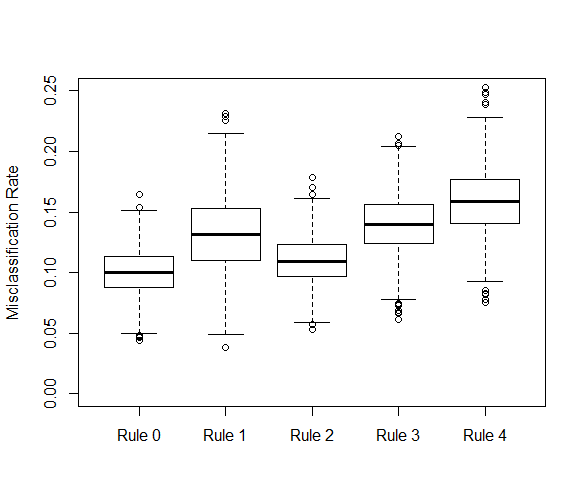
\includegraphics[scale=0.8]{Photos/Mis rates.png}
    \captionsetup{justification=centering}
    \caption{Synthetic misclassification rates without retake for the rules in Table \ref{tab:Amend}, over 1000 datasets.}
    \label{fig:Decisions}
\end{figure}
\end{document}